%!TEX root = ../main.tex
%%%%%%%%%%%%%%%%%%%%%%%%%%%%%%%%%%
% Links: https://leetcode.com/problems/find-minimum-in-rotated-sorted-array/
%
% Difficulty: Medium
% Companies: 
%%%%%%%%%%%%%%%%%%%%%%%%%%%%%%%%%%

\chapter{Minimum element in rotated sorted array}
\label{ch:min_rotated_array}
\section*{Introduction}
The problem described in this chapter is a very popular interview question that has a surprisingly short statement in length and has a very obvious linear time solution. But, despite being quite short and having a trivial  brute-force solution, solving this problem efficiently is not easy and requires a bit of thinking and careful coding to implement it elegantly. 

\section{Problem statement}
\begin{exercise}
Given a ascending sorted array with no duplicates and rotated around a pivot, return the minimum element.
\end{exercise}


\begin{example}
	\hfill \\
	Given the rotated array $\{3,4,5,6,1,2\}$ the function returns $1$
\end{example}

\begin{example}
	\hfill \\
	Given the rotated array $\{0,2,3\}$ the function returns $0$
\end{example}

\begin{example}
	\hfill \\
	Given the rotated array $\{3,2,1\}$ the function returns $1$
\end{example}

\section{Clarification Questions}

\begin{QandA}
	\item Are all the elements unique? 
	\begin{answered}
		\textit{Yes, you can assume all the elements are unique}
	\end{answered}
	\item Can the input array be empty?
	\begin{answered}
		\textit{No, you might assume the array contains at least one element.}
	\end{answered}
\end{QandA}

\section{Discussion}
\label{min_rotated_array:sec:discussion}
What does it really mean for a sorted array to be rotated around an element? Given a sorted array $A=\{a_0, a_1, \ldots,a_{n-1}\}$ s.t. $ \forall \: 0 \leq i < n: a_i < a_{i+1}$, rotating A around the pivot element at index $p$ results in: $A_p=\{a_p, a_{p+1}, \ldots,a_{n-1}, a_0, a_1, \ldots, a_{p-1}\}$. In  nutshell all the elements are rotated in such a way that the element at index $p$ becomes the first element of the array. For instance, rotating the array $X=\{1,2,3,4,5\}$ around the element at index $2$, results in $X=\{3,4,5,1,2\}$.  There is also an array rotation algorithm in the C++ STL\cite{cit::std::rotate}.


\subsection{Brute-force}
\label{min_rotated_array:sec:bruteforce}
The brute force is trivial and consist in simply looping through the array and keeping record of the smallest element encountered. In C++ this can be implemented with a one-liner as shown in Listings \ref{list:min_rotated_array_bf} and \ref{list:min_rotated_array_bf_manual}.
Both implementations have a $O(n)$ time and constant space complexity.

\lstinputlisting[language=c++, caption=One-linear brute force (using C++ STL) solution to the problem of finding the minimum element in a sorted rotated array.,label=list:min_rotated_array_bf]{sources/min_rotated_array/min_rotated_array_solution1.cpp}

\lstinputlisting[language=c++, caption=One-linear brute force solution to the problem of finding the minimum element in a sorted rotated array.,label=list:min_rotated_array_bf_manual]{sources/min_rotated_array/min_rotated_array_solution2.cpp}

This approach should just be mentioned during the interview but no time should be spent in the actual implementation of this idea, as the interviewer is assuming you know how to trivially search for the minimum in an unsorted array. He is clearly looking for a more advanced solution that takes advantage of the fact that the array is sorted (even if rotated).

\subsection{Logarithmic solution}
\label{min_rotated_array:sec:log}
As usual, when in the problem statement the word "sorted" makes its appearance the first thought that should cross our brain is: \textbf{binary search}(see Appendix \ref{sect:appendix:binary_search}). In this case, we are almost forced to think about binary search immediately as the problem is about searching the word sorted is mentioned in the statement. So, binary search can be employed to solve this problem. The idea is simple, as for all the binary search application we need to:

\begin{enumerate}
	\item keep track of a range of element that are currently under examination. Initially this range is the following closed interval: $[l=0, r=A.size()-1]$
	\item analyze the element on the middle of this range.
	\item if the middle element is the element we are looking for we are done
	\item otherwise, the search proceed either to the left or to the right or the range. 
\end{enumerate}

The key point of this problem lies at steps $2$ and $3$ because we need to be able:
\begin{itemize}
	\item $2$ test whether an element is the minimum or not
	\item $3$ decide how to split the space range into two and whether proceed the search on the right-hand or on the left-hand side.
\end{itemize}

\subsubsection{Test if an element is the minimum}
In order to decide whether an element $a_k$ at index $k$ is the minimum in our array i.e. our answer it is useful to look at one property that differentiates it from all the other values in the collection. The minimum element is the only element s.t. both the elements on its right and left are \textbf{greater} than it (this element is also called inflection point). Another other useful property that can be helpful in the identification of the minimum is that the element on its left it is always the maximum element of the array (see examples in the Section \ref{min_rotated_array:sec:discussion} and Figure \ref{fig:min_rotated_array:test_element}). Thus whenever $a_{k-1} > a_{k}$ (meaning that $a_k$ is the minimum and $a_{k+1}$ the maximum) or $a_{k} > a_{k+1}$ (meaning that $a_k$ is the maximum element and $a_{k+1}$ the minimum) we can stop and return because we have found the answer. 

\begin{figure}
	\label{fig:min_rotated_array:test_element}
	\centering
	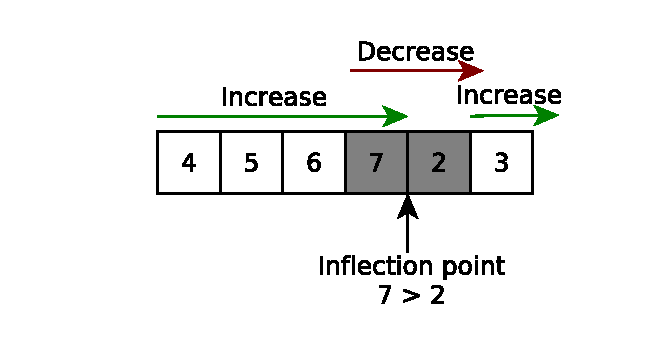
\includegraphics[scale=1.0]{sources/min_rotated_array/images/inflection_point}
	\caption{Inflection point in a rotated sorted array. When the binary search examines both element $7$ and $2$ it is able to determine the inflection point (element $2$). }
\end{figure}

In short, Listing \ref{list:test_answer} shows the condition that can be used in the binary search to test whether $a_k$ is the answer to the problem. Please note how in order to avoid having special cases for the elements at the beginning 

\begin{lstlisting}[language=c++, caption={Test to verify whether the binary search can stop because an answer has been found.},label=list:test_answer]]{
	const int curr = A[k];
	//+A.size() due to negative modulo
	const int prec = A[(k-1+A.size())
	const int succ = A[(k+1)%A.size()];
	if( (curr <= prec ) || (curr >= succ))
		return min({prec , curr , succ});
}
\end{lstlisting}

\subsubsection{Binary search range split}
The last part of the algorithm that still need to be figured out is how to continue the search in the case the element in the middle of the range is not good to determine the answer. A nice property of the sorted rotated array is that if the answer is at position $i$ then \textbf{all the element on the right side of it are smaller than the very first element of the array} i.e. the following is always true:
\begin{itemize}
	\item[-] $	(a_i < a_0) \: \wedge (a_{i+1} < a_0) \: \wedge \ldots (a_{n-1} < a_0) $
	\item[-] $	(a_{i-1} \geq a_0) \: \wedge \: (a_{i-2} \geq a_0) \: \wedge \: \ldots \: (a_{0} \geq a_0) $
\end{itemize}
This is the last piece of information that is needed in order to have the binary search working. Given an element at position $i$ that is not the answer we  will search on the left-hand side of $i$ if $a_i > a_0$, otherwise we will use the right side.


The idea above can be implemented as shown in the Listing \ref{list:min_rotated_array_log}. This solution as a complexity of $O(log(n))$ time and $O(1)$ space.

\lstinputlisting[language=c++, caption={Logaritmic solution to the problem of finding the minimum element in a sorted and rotated array.},label=list:min_rotated_array_log]{sources/min_rotated_array/min_rotated_array_solution3.cpp}
